\documentclass{report}

\input{../template/preamble}
\input{../template/macros}
\input{../template/letterfonts}

\title{\Huge{Magnetism}\\Semester 5}
\author{Ahmad Abu Zainab}
\date{}

\begin{document}

\maketitle
\newpage% or \cleardoublepage
% \pdfbookmark[<level>]{<title>}{<dest>}
\pdfbookmark[section]{\contentsname}{toc}
\tableofcontents
\pagebreak

\chapter{Electromagnetic Waves}

Electromagnetic waves are waves that are created by oscillating electric and magnetic fields. The electric and magnetic fields are perpendicular to each other and to the direction of propagation of the wave.
They travel at a speed of $c=299792458$ \unit{m/s} in a vacuum. The frequency of the wave is given by $f=\frac{c}{\lambda}$ where $\lambda$ is the wavelength of the wave.

The wavelength is the distance between two consecutive peaks of the wave.

\begin{figure}[ht]
	\centering
	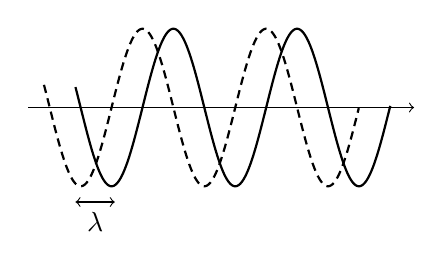
\begin{tikzpicture}[domain=-4:0]
		\draw[->] (-4.2,0) -- (0.7,0);

		\draw[smooth,thick, samples=1000, densely dashed]   plot (\x,{sin(4*\x r)});
		\draw[smooth,thick, samples=1000, domain=-3.6:0.4]   plot (\x,{sin(4*\x r - 90)});
		\draw[<->] (-3.6,-1.2) -- (-3.1,-1.2) ;
		\draw (-3.35,-1.2) node[below] {$\lambda$};
	\end{tikzpicture}
\end{figure}

The wave moves a distance $x$ in a time $t$ with a speed
\[
	v = \frac{x}{t} = \frac{\omega}{k} = \frac{\lambda}{T} = \lambda f
	.\]

\[
	\lambda = \frac{2\pi}{f}
	.\]

The equation of the wave is given by

\[
	y = A\sin \lt( \omega t - kx + \phi \rt)
	.\]

The intensity of the wave is given by

\[
	I = \frac{P}{4 \pi r^2}
	.\]

\subsection{Poynting Vector}

The Poynting vector is a vector that represents the energy flux of the wave. It is given by

\[
	\va{S} = \frac{1}{\mu_0}\va{E} \times \va{B}
	.\]

However, since $\va{B}$ are perpendicular to $\va{E}$ then

\[
	S = \frac{1}{\mu_0}EB
	.\]

and since

\[
	c = \frac{E}{B}
	.\]

then

\[
	S = \frac{c}{\mu_0}B^2 = \frac{1}{c\mu_0}E^2
	.\]

\subsection{Maxwell's Equations}

\begin{align*}
	\pdv{\va{E}}{x} & = - \pdv{\va{B}}{t}                     \\
	\pdv{\va{B}}{x} & = - \varepsilon_0 \mu_0 \pdv{\va{E}}{t}
\end{align*}

\chapter{Optics}

The equation of an EM wave is given by

\[
	\va{E} = E_0 \sin \lt( \omega t - kx \rt) \vu{\jmath}
	.\]

Noting that electric field typically have all directions, whenever an non-polarised electric field hits a polariser, only the electric field components that are along the line of polarization are allowed to pass while all others are absorbed. If the electric field direction is perpendicular to the line of polarization then it is entirely absorbed while the electric field vectors that have an angle $\theta <\pi /2$ then only the projection of that vector on the polarization line will not be absorbed.

Given a polariser with angle $ \alpha $ then the electric field $\va{E } $ hitting that polariser has an equation

\[
	\va{E} = \underbrace{E \sin \alpha\vu{u}_1}_{\text{transmitted}} + \underbrace{E\cos \alpha\vu{u}_2}_{\text{absorbed}}
	.\]

\subsection{Reflection}

The angle of incidence is equal to the angle of reflection.

\[
	\theta_i = \theta_r
	.\]

\begin{figure}[H]
	\centering
	\begin{tikzpicture}
		\draw[->,thin] (-4,0) -- (4,0);
		\draw[->,thin] (0,0) -- (0,4);
		\draw[-{Latex},thick] (0,0) -- (2,2) node[above] {$\va{E}_i$};
		\draw[-{Latex},thick] (-2,2) node[above] {$\va{E}_r$} -- (0,0);
		\draw (0,0.5) arc (90:135:0.5) node[midway,above] {$\theta_i$};
		\draw (0,0.5) arc (90:45:0.5) node[midway,above] {$\theta_r$};
	\end{tikzpicture}
\end{figure}


\subsection{Refraction}
Snell's law
\[
	n_1\sin \theta_1 = n_2\sin \theta_2
	.\]

\begin{figure}[H]
	\centering
	\begin{tikzpicture}
		\draw[thin] (-3,0) -- (3,0);
		\draw[thin, dashed] (0,-2.7) -- (0,2.7);
		\draw[-{Latex},thick] (-2,2) -- (0,0);
		\draw[-{Latex},thick] (0,0) -- (1,-3);
		% Draw the angle 
		\draw (0,0.6) arc (90:135:0.6) node[midway,above] {$\theta_1$};
		\draw (0,-0.6) arc (-90:-73:0.6) node[midway,below] {$\theta_2$};
		\draw (3,1) node[above] {$n_1$};
		\draw (3,-1) node[above] {$n_2$};
	\end{tikzpicture}
\end{figure}

This implies that if $n_1 < n_2$ then $\theta_1 > \theta_2$.


\dfn{Critical Angle}{
	The critical angle the maximum angle of refraction where the refracted ray goes back in the incident medium

	\[
		\theta_c = \sin^{-1} \lt( \frac{n_2}{n_1} \rt)
		.\]
	\begin{figure}[H]
		\centering
		\begin{tikzpicture}
			\begin{scope}[xshift=-3cm, scale=0.75]
				\draw[thin] (-3,0) -- (3,0);
				\draw[thin, dashed] (0,-2.7) -- (0,2.7);

				\draw[-{Latex},thick] (-1.5,-1.5) -- (0,0);
				\draw[-{Latex},thick] (0,0) -- (2,0);

				\draw (2,1) node[above] {$\theta_1=\theta_c$};
				\draw (2,-1) node[above] {$\theta_2=\ang{90}$};

				\draw (0,-0.5) arc (-90:-135:0.5) node[midway,below] {$\theta_1$};
				\draw (0,0.5) arc (90:0:0.5) node[midway,above] {$\theta_2$};
			\end{scope}
			\begin{scope}[xshift=3cm, scale=0.75]
				\draw[thin] (-3,0) -- (3,0);
				\draw[thin, dashed] (0,-2.7) -- (0,2.7);

				\draw[-{Latex},thick] (-2.5,-1) -- (0,0);
				\draw[-{Latex},thick] (0,0) -- (2.5,-1);

				\draw (-2,1) node[above] {$\theta_1>\theta_c$};

				\draw (0,-0.5) arc (-90:-158.2:0.5) node[midway,below] {$\theta_1$};
				\draw (0,-0.5) arc (-90:-21.8:0.5) node[midway,below] {$\theta_2$};
			\end{scope}

		\end{tikzpicture}
	\end{figure}
}

\[
	v = \frac{c}{n}
	.\]

\begin{align*}
	\text{Speed of light in a medium} & = \frac{1}{\sqrt{\mu \varepsilon}}     \\
	\text{Speed of light in a vacuum} & = \frac{1}{\sqrt{\mu_0 \varepsilon_0}} \\
	\text{Refractive index}           & = \sqrt{\mu_r \varepsilon_r}
\end{align*}


\[
	\frac{n_1}{n_2} =\frac{v_2}{v_1}
	.\]

\end{document}
